\documentclass{standalone}

\usepackage{tikz}

\begin{document}
  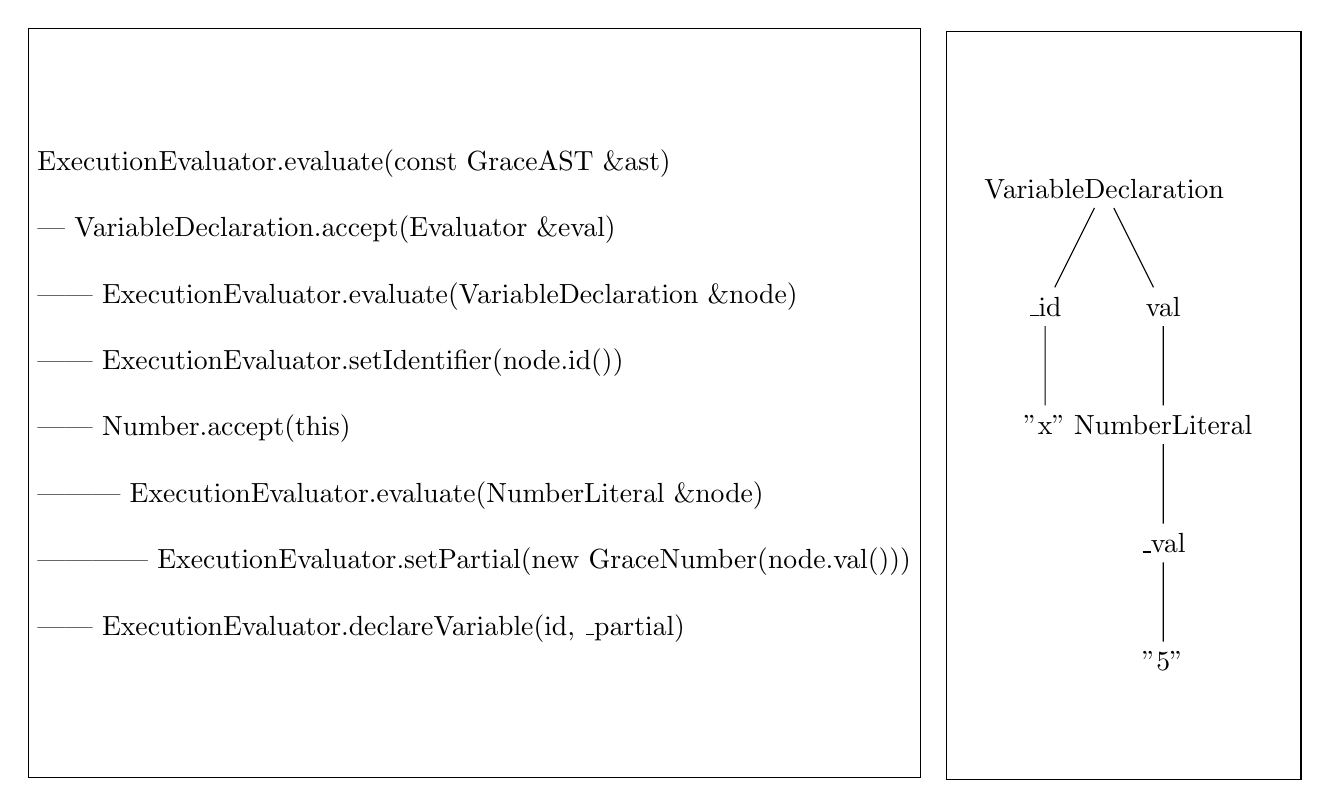
\begin{tikzpicture}
  	\node[draw,align=left] at (0,-0.72) {\\ \\ \\ \\
ExecutionEvaluator.evaluate(const GraceAST \&ast)\\ \\ | VariableDeclaration.accept(Evaluator \&eval)\\  \\ || ExecutionEvaluator.evaluate(VariableDeclaration \&node)\\ \\  || ExecutionEvaluator.setIdentifier(node.id())\\   \\  || Number.accept(this)\\ \\     ||| ExecutionEvaluator.evaluate(NumberLiteral \&node)\\   \\    |||| ExecutionEvaluator.setPartial(new GraceNumber(node.val()))\\  \\   || ExecutionEvaluator.declareVariable(id, \_partial) \\ \\ \\ \\   	};

	\draw  (6,4) rectangle (10.5,-5.5);
	\node at (8, 2) {VariableDeclaration} [grow'=down]
		child {node {val}
			child {node {NumberLiteral}
				child{node{\_val}
					child{node{"5"}}
				}
			}
		}
		child {node {\_id}
			child {node {"x"}}		
	};
\end{tikzpicture}
\end{document}